\documentclass[hidelinks,conference,12pt]{IEEETran}
\usepackage[english]{babel}
\usepackage{graphicx}
\usepackage{tabularx}
\usepackage[backend=bibtex, natbib=true]{biblatex}
\usepackage{listings}
\usepackage{multicol}
\usepackage{hyperref}
\usepackage{placeins}
\usepackage{amssymb}
\usepackage{fancyhdr}

\pagestyle{fancy}
\fancyhf{}

\rfoot{Page \thepage \hspace{1pt} of 15}
\bibliography{bibliography}
\setlength{\parindent}{0in}
\pagenumbering{arabic}


\title{HIS Safety Critical Systems - Human Activity Recognition \\ Fall Detection based on Accelerometer and Gyroscope Data}
\author{
	 Anton Beck \\ 952857
\and Muyassar Kokhkharova \\ 1248560
\and Xhoni Robo \\ 1248434
}

\begin{document}

\maketitle

\begin{abstract}

This is the final report for the group project for the High Integrity Systems M.Sc. Safety Critical Systems for the Winter Semester 2018/2019, lead by Prof. Dr. Matthias F. Wagner. Here Group A, composed from the authors of this report, will present the effort and results of the work put into this project.\textsuperscript.\\
The application is supposed to take data received from three sensors, two accelerometers and one gyroscope, and detect using calculations based on this data whether the subject has fallen or not. The data is represented by text files given to the students by Assistant Professor Luigi La Blunda.{\cite{lablunda}}\\
The project spanned seven weeks (not counting holidays), from the beginning of the semester to the 15th of February 2019.\\
The report is meant to accompany the application and may be used as documentation. However, the elements covered here will include not just those related to the application itself, but also more importantly the process and different steps and strategies that went into the project. This includes things like the original plan and the hardships the members faced as well.\\
All the deliverables of this group project are part of the work of the group members. Whenever an external resource is used, it will be cited accordingly. The exemption is open source elements that are well known and commonly used by everyone (e.g. Java Libraries)\\
The project is as of the date of delivery of this report considered finished. The team members are not to be held accountable for any of the following past the date specified above:
\begin{itemize}
	\item maintenance and support of the product
	\item a user manual
	\item hardware
\end{itemize}
Note: The group had one more member who in the end decided to change his degree and not proceed with the project. As they are no longer part of the group, their name will not be included in this report. 	
\end{abstract}

\section{Functional and Non-Functional Requirements}
\subsection{Functional Requirements}
\begin{enumerate}
	\item A PC application that takes in .txt files as input.
	\item The application should analyse the data and detect whether there was a fall.
	\item The data from the file must be visualized.
	\item Main UI with basic control functions for operator working with a PC application.
	\item Application allows the user to enter their data
	\item Application allows the user to change different settings pertaining to the fall detection.
	\item Application can differentiate between falls and fall like activities.
\end{enumerate}


\subsection{Non-Functional Requirements}
\begin{enumerate}
	\item Pop-up window containing the following User settings:
	\begin{itemize}
		\item First Name
		\item Last Name
		\item Date of Birth
		\item Gender
		\item Address
		\item Mobile phone number of the User
		\item Blood Type
		\item Contact Person (In case of a fall this Person will be contacted.)
		\item Contact Email (Email of the Contact Person.)
		\item Save button to save the changes
	\end{itemize}
	\item Pop-up window containing the following application settings:
	\begin{enumerate}
		\item Values of Impact (in g)
		\item Measurements after Impact
		\item Laying Acceleration (in g)
		\item Skipped Measurements
		\item Fall Angle (in $^{\circ}$)
		\item Measurements per Second
		\item Lower Laying Limit (in g)
		\item Upper Laying Limit (in g)
		\item Accelerometer Scale
		\item Help Request Delay (in mS)
	\end{enumerate}
	\item In Main UI:
	\begin{enumerate}
		\item Graphs with Accelerometer and Gyroscope data.
		\item Button Browse to select a .txt file.
		\item Buttons Start/Stop to start/stop the data reading process.
		\item Label for Fall Detection.
		\item Label for "Help requested"
		\item "False Alarm" Button (for testing purposes)
		\item Fall Button (for testing purposes)
	\end{enumerate}
\end{enumerate}

\subsection{Safety, Security and Reliability Requirements}
As the name of the course that this report is written for implies, safety, security and reliability of this application are to be considered throughout the whole process of making this application. An error or miscalculation could mean the difference in the detection of a fall. \\
While this project is not meant to be used in real applications, but rather give the user a simple way of testing the effects of different parameters in order to find the best formula for fall detection based on the given sensor data, missing a key element, regardless of how small it may be, could lead to the formula being incorrect and later on result in faulty programs based on this application. If a program that is meant to be applied to a real scenario, such as for example the monitoring of the elderly in a retirement home, a false alarm could mean massive costs (e.g. calling emergency services incorrectly), while a missed fall could mean the loss of human life.\\
For safety, we need too ensure that the different software mechanisms that are used to detect a fall are well protected. Our current application uses local text files that have a very specific format. While the program cannot run with files that are not formatted properly, incorrect data could easily cause the model to function improperly. Since we use the difference in acceleration and rotation forces to detect a fall, a single outlying value could possibly cause a fall where there should not be one.\\
As far as security is concerned, we make the assumption that the user of the application has experience in the field. That means that the user knows not only how to use the provided data, but also how to change the different settings to improve his analysis. To ensure that the application does not cause security concerns outside of user error, we implement some fault tolerance protocols, such as outright not allowing the user to do certain erroneous actions.\\
For reliability, we want the application to only detect falls. There are many activities that have distinct yet similar patterns to a fall. The more the application can differentiate between these actions, the more reliable it becomes. Lastly, we take an extra step and send a notification by email. This logic can be replaced with any other contact method that is faster and perhaps more reliable, as long as it always works. Below is the full list of safety, security and reliability requirements:\\

\subsubsection{Safety Requirements}

\begin{enumerate}
	\item Software correctly notifies when a person has fallen
	\item User can press a button to notify a False Alarm
\end{enumerate}

\subsubsection{Security Requirements}

\begin{enumerate}
	\item The components that the application uses as the base of its logic are hidden from the user. User interacts only through the use of UI
	\item The user can only submit properly formatted data, otherwise the application will not proceed
\end{enumerate}

\subsubsection{Reliability Requirements}

\begin{enumerate}
	\item The application is able to differentiate between falls and other activities
	\item The application can run for long periods of time and is able to read the whole text file
	\item On fall detection, ensure a notification is always sent, provided it is not a False Alarm
\end{enumerate}

\section{Project Planning}

\subsection{Project Estimation}
In order to estimate the effort required for this project, we used the COCOMO II model\textsuperscript{\cite{cocomo}} that uses Function Points\textsuperscript{\cite{albrecht}} to calculate effort. A summary will be presented below.

\subsubsection{Function Points}
We use the Function Points calculation process until the Unadjusted Function Point values are obtained, as these are the values used in the COCOMO II model.\\
For the purposes of this calculation, we consider the application to be a conglomeration of separate components (different modules with individual tasks), rather than a singular system. While these modules are separate, the internal communication between them cannot be considered a transaction. This, coupled with the fact that the system as a whole is a stand-alone program, means we do not have to consider External Interface Files.

\FloatBarrier
\begin{table}[h]
	\centering
	\caption{\textbf{Function Points Calculation}}
	{\renewcommand{\arraystretch}{2}%
		\begin{tabular}{|l|p{1cm}|}
			\hline
			 & FP \\
			\hline
			External Input & 29 \\
			\hline
		    External Output & 24 \\
		    \hline 
			External Inquiry & 21 \\
			\hline
			Internal Logical Files & 7 \\
			\hline
			Total & 81 \\
			\hline
	\end{tabular}}
\end{table}
\FloatBarrier

From the above calculation we have thee following estimation from the COCOOMO II model:

\FloatBarrier
\begin{table}[h]
	\centering
	\caption{\textbf{Function Points Calculation}}
	{\renewcommand{\arraystretch}{2}%
		\begin{tabular}{|l|p{1cm}|}
			\hline
			Person-Months & 7.4 \\
			\hline
			Schedule Months & 1.5 \\
			\hline
			SLOC & 4293 \\
			\hline 
	\end{tabular}}
\end{table}
\FloatBarrier
This is our final estimation, which is identical to our original one.

\subsection{Group Organization}

In organizing the group, there were many factors to consider. Firstly, the project spans a relatively short amount of time. On top of the strict deadline, the members are supposed to complete exercises throughout the semester to aid them in the delivery of the project. This time crunch is made even worse by the fact that the members not only have other courses to study for, but also employment obligations. As such, the group decided on adopting an agile development strategy. Every two weeks the members would hold a scrum meeting on Thursdays at 15:30 to discuss the progress of the project and the tasks for the next sprint. The exception to the above was on two occasions before and after the Winter break, where the members met and worked physically together on the code of this application.\\
For official communication we used:
\begin{itemize}
	\item important messages were sent through the Slack\textsuperscript{\cite{slack}} "SCS" group chat
	\item general communication unrelated to the coding aspects was done through WhatsApp\textsuperscript{\cite{whatsapp}}
	\item in case of communication with the professor or assistants of the project, we used Moodle\textsuperscript{\cite{moodle}} or email
\end{itemize}
Slack is particularly useful due to the fact that we can connect a GitHub repository. Whenever one of the members made changes to the code, the whole group would receive a message. The project files, including all the work done throughout the semester as well as this documentation is included in the GitHub repository\textsuperscript{\cite{github}} that the team used to coordinate.

\subsection{Responsibilities of the Team Members}

For the sake of professionalism, each team member is assigned a main role. What this means is that the respective member will lead the efforts in that one area that they are assigned to. However, this does not imply that the work load separation will follow this pattern. \\
The members could and did take multiple roles throughout the course of the project, as this made it possible to assign more importance to certain tasks that would otherwise take too long to complete. Below are the areas in which the members were separated. With one team member leaving the group before the end (not included), the roles changed minutely for the last two weeks of the project span. 
\FloatBarrier
\begin{table}[h]
	\centering
	\caption{\textbf{Roles of the Team Members}}
	{\renewcommand{\arraystretch}{2}%
		\begin{tabular}{ | l | l | }
			\hline
			\textbf{Name} & \textbf{Main Role} \\ \hline
			Anton Beck & Mathematical Model \\ \hline
			Muyassar Kokhkharova & Statistics, UI Designer \\ \hline
			Xhoni Robo & Project Manager, Java Developer \\ \hline 
	\end{tabular}}
\end{table}

\subsection{Schedule}
The original team plan was to have a finished demo application containing only the basics necessary to make it work by latest end of January. \\
The plan was followed through successfully up until after the Winter break, where one of the team members decided not to continue with the project. At that point, the only task left to be completed was putting the separate parts of the application together and making it run fluently.\\
 Suddenly being down a member delayed the progress by two weeks, as the remaining members had to first understand the code that was already written there by the abandoning member, and then proceed to finish the task. There was a chance that the project would not be completed on time, however due to a lot of effort from the remaining members the application was ready on time. 

\clearpage
\FloatBarrier
\subsection{Project Risk Analysis}
\FloatBarrier
\begin{figure}[!h]
	\centering
	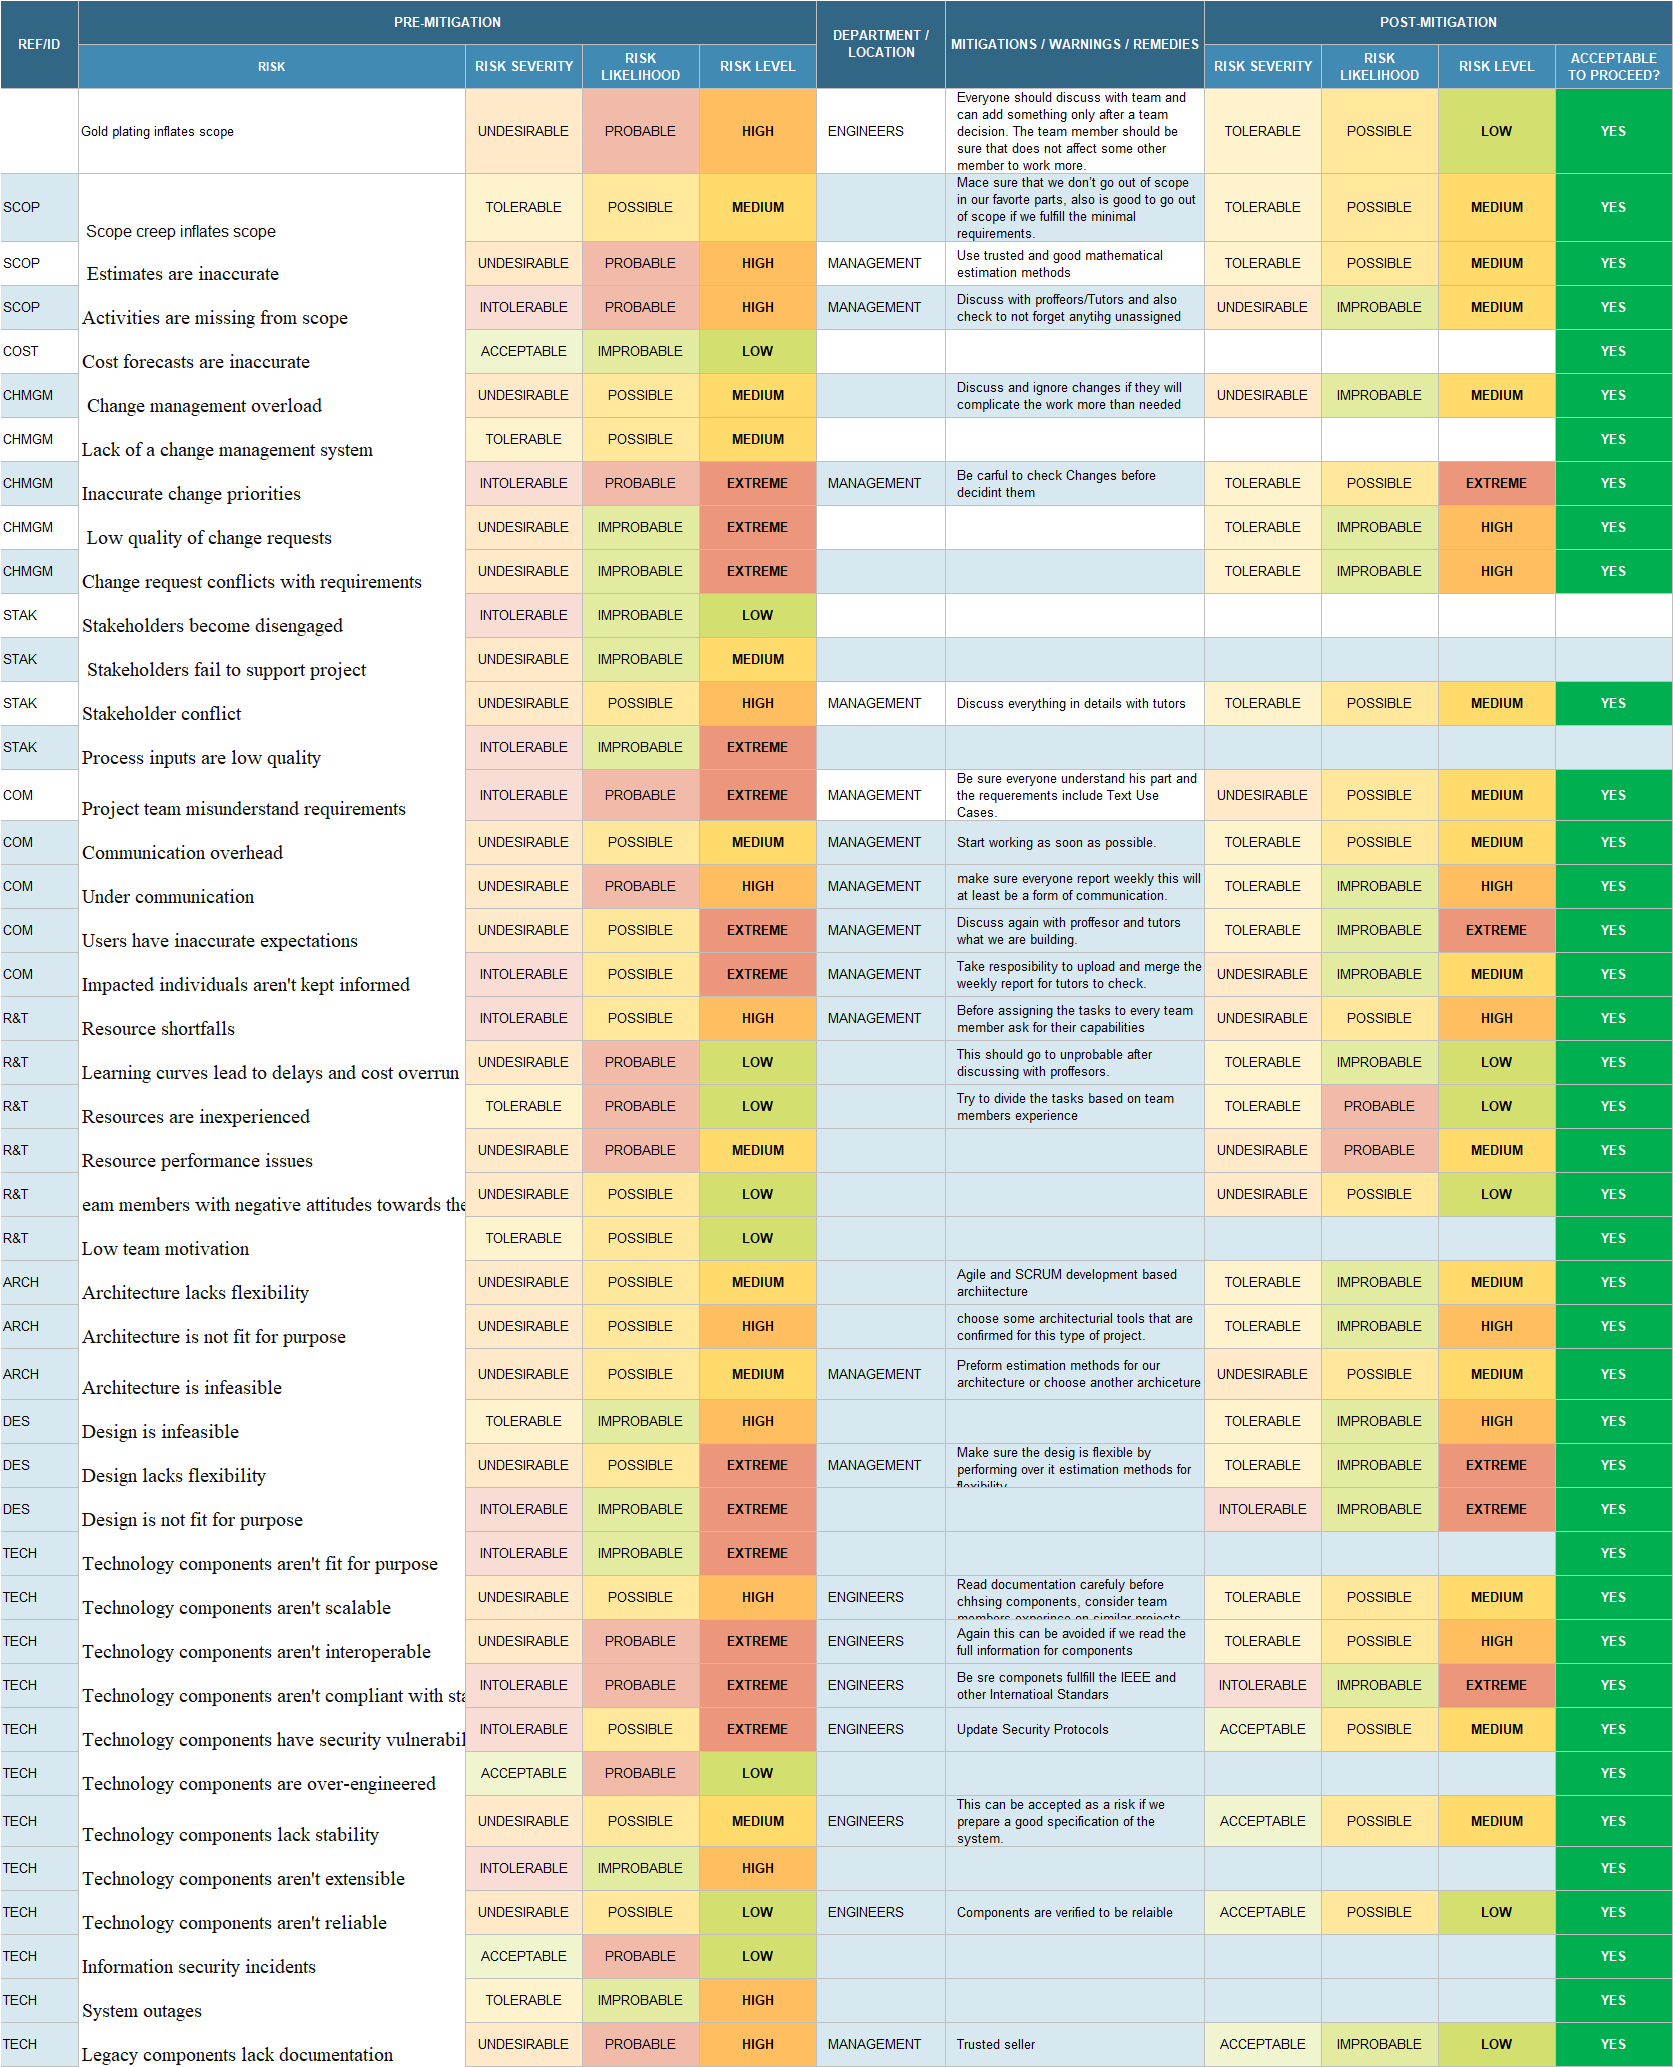
\includegraphics[scale=0.39]{images/Risk_Man_Matrix.png}
	\caption{Risk Management Matrix}
	\label{img:Risk_Man_Matrix}
\end{figure}
\FloatBarrier

\clearpage

\FloatBarrier
\begin{figure}[!h]
	\centering
	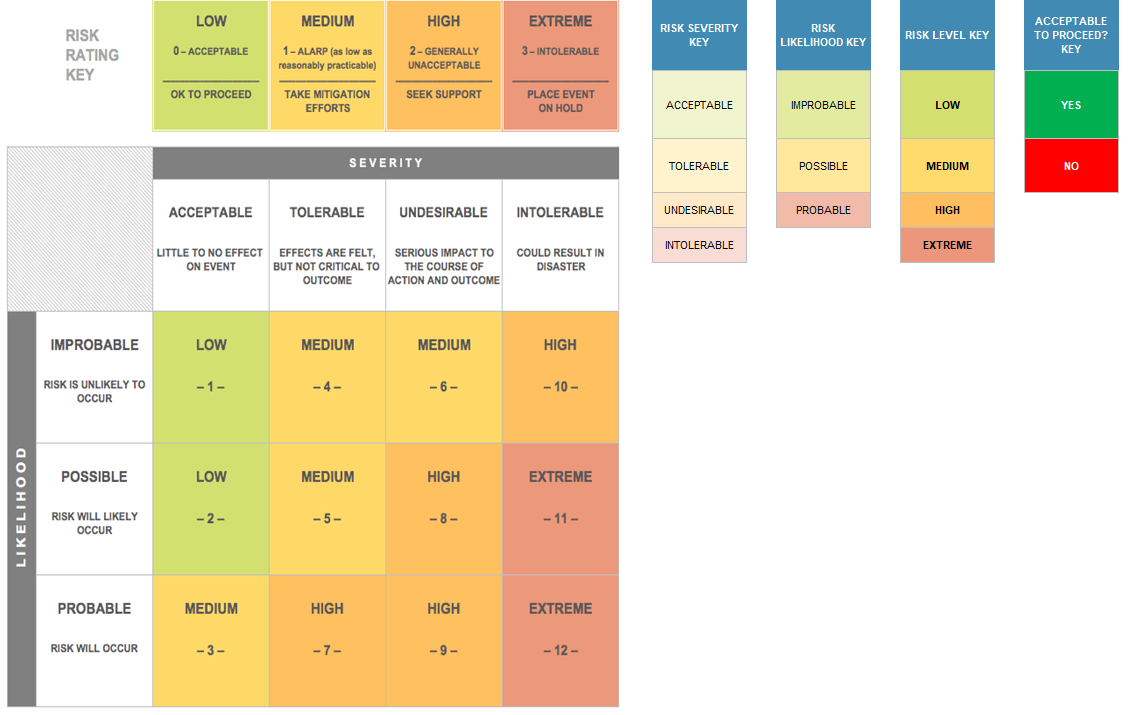
\includegraphics[scale=0.6]{images/Risk_Man_Key.png}
	\caption{Risk Management Matrix Key}
	\label{img:Risk_Man_Key}
\end{figure}
\FloatBarrier
	
\clearpage

\section{Design}
\subsection{Use Case Diagram}

\textit{System Start}: User selects a .txt file and presses the Start button\\
\textit{Recognises Fall}: Application detects a spike in acceleration, confirms with rotation data and then alerts the user of a fall\\
\textit{Receiving False Alarm}: If the False Alarm button is pressed within ten seconds(configurable) of a fall event, no notification is sent. If pressed after ten seconds, a follow up notification is sent after the fall notification, notifying the user that the previous message was a false alarm\\
\textit{Personal data changes}: Allows the user to change the personal data of the person to be contacted\\
\textit{Calibration changes}:  Allows the user to change the parameters that are used in the calculation of a fall\\\\\\\\\\

\FloatBarrier
\begin{figure}[!h]
	\centering
	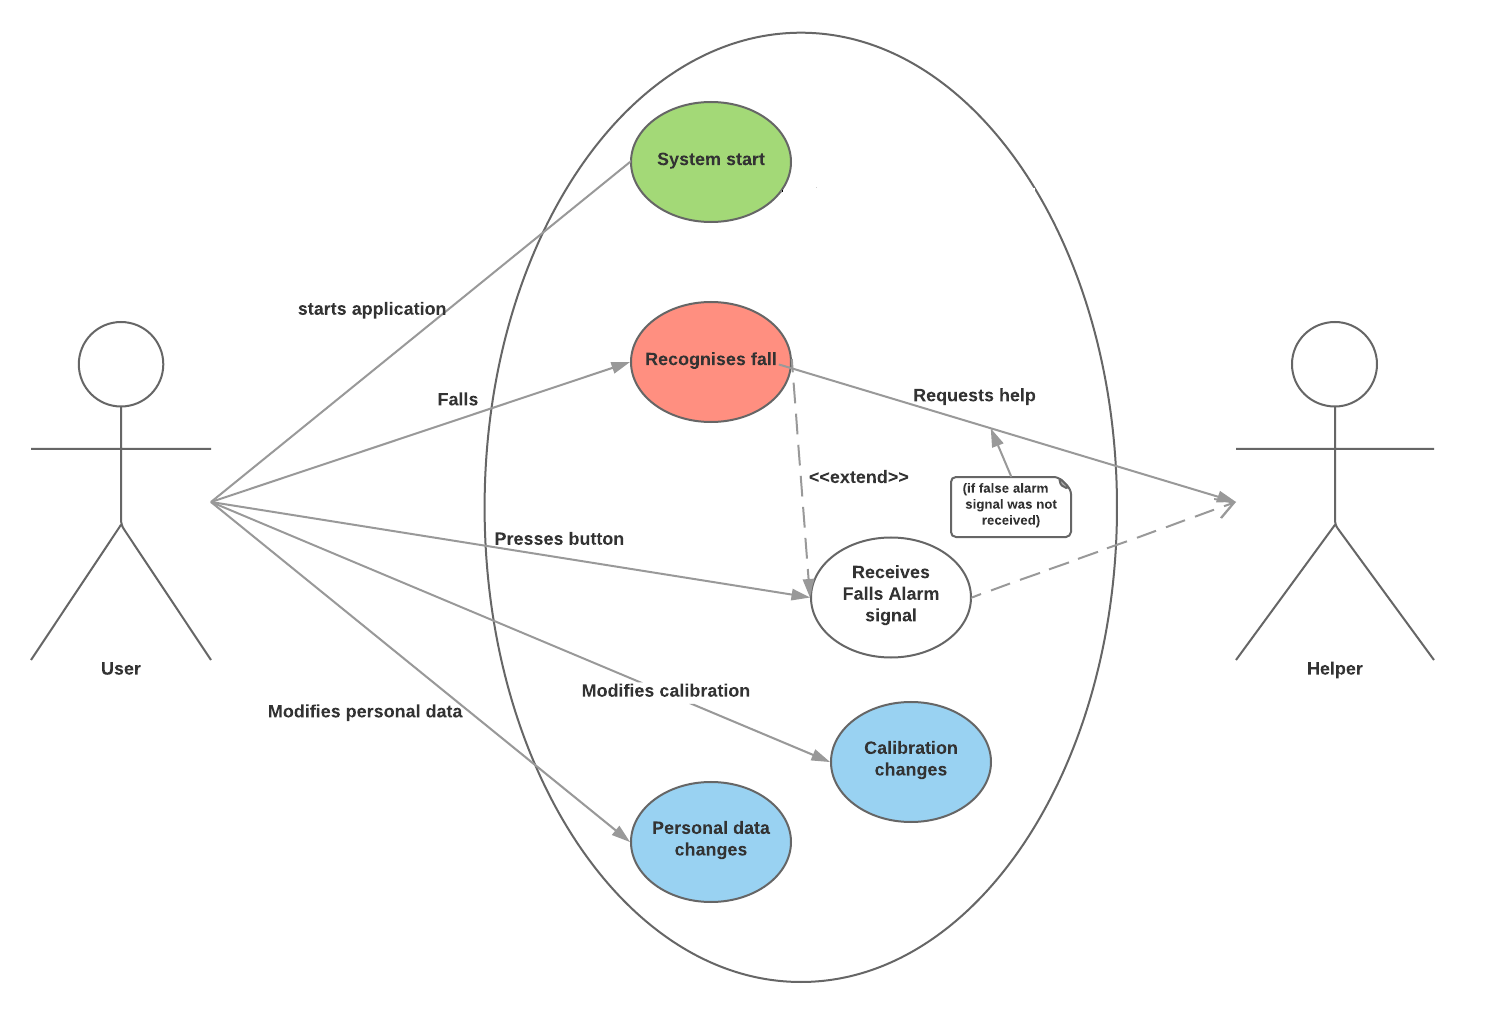
\includegraphics[scale=0.23]{images/Use_Case_Diag.png}
	\caption{Use Case Diagram\textsuperscript{\cite{umlspec}}}
	\label{img:Use_Diag}
\end{figure}
\FloatBarrier
\vskip 3cm
\subsection{Sequence Diagrams taken from the Use Cases}
To better explain the Use Case Diagram, a sequence diagram is included below.

\FloatBarrier
\begin{figure}[!h]
	\centering
	\caption{System Start}
	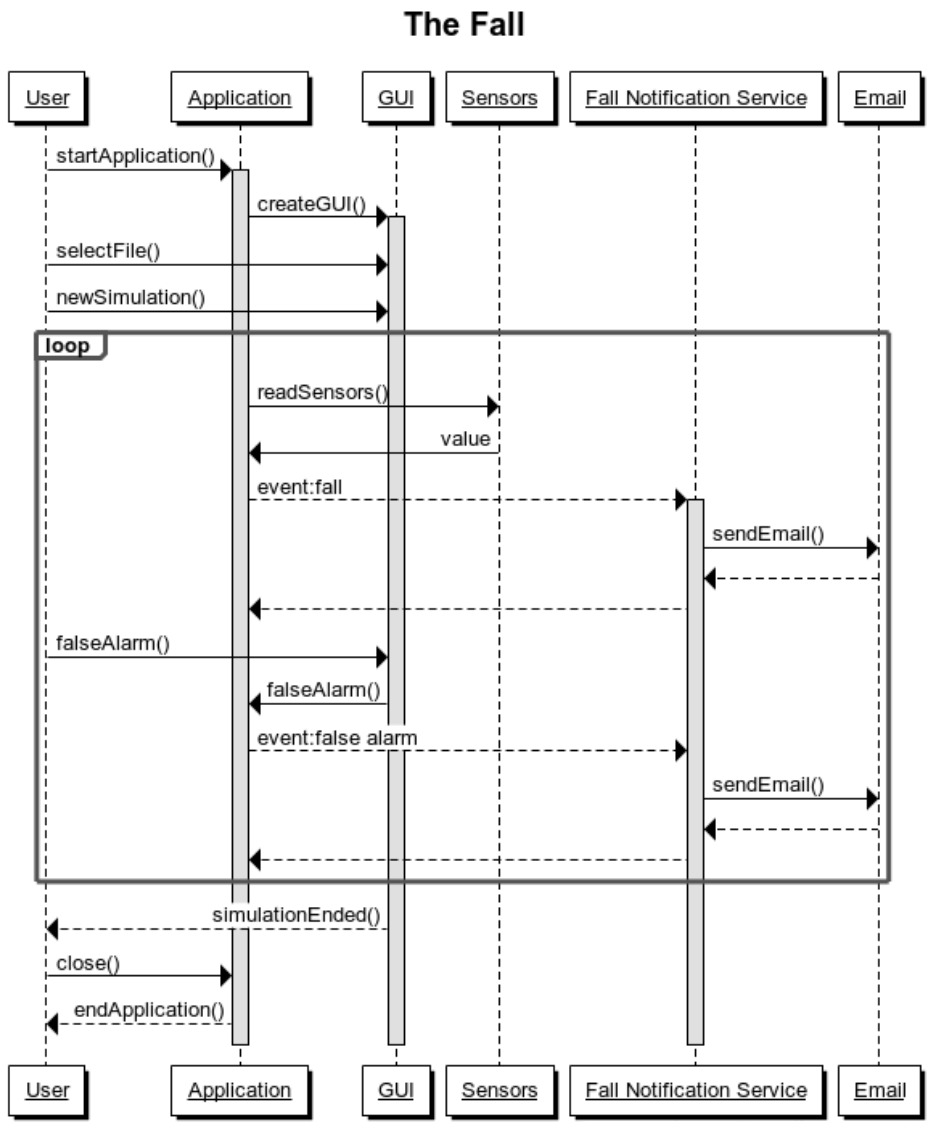
\includegraphics[scale=0.29]{images/Seq_Diag.jpeg}
	\label{img:start}
\end{figure}
\FloatBarrier

\subsection{Software Architecture}
For our project, we decided to use a Layered Architecture that separates the classes into different packages based on the responsibilities of each individual class. This separation was done manually by the group members, without using any inbuilt or open source software or framework.
Most classes can only communicate with the classes in their own package. Each package has a class that behaves as an entry point for the layer above and below. For example, the top level layer is the User Interface Layer. It may only directly communicate with the layer below it, the Application Logic Layer, which in turn communicates with the Mathematics and Notification Layers below it.
 For a Fall event, the notification must first pass through the Application Logic Layer to get to the User Interface Layer. Not only is this code separation helpful in lightening the complexity of the application, it also improves cohesion between classes. \\
 
 \FloatBarrier
 \begin{figure}[!h]
 	\centering
 	\caption{UML Diagram}
 	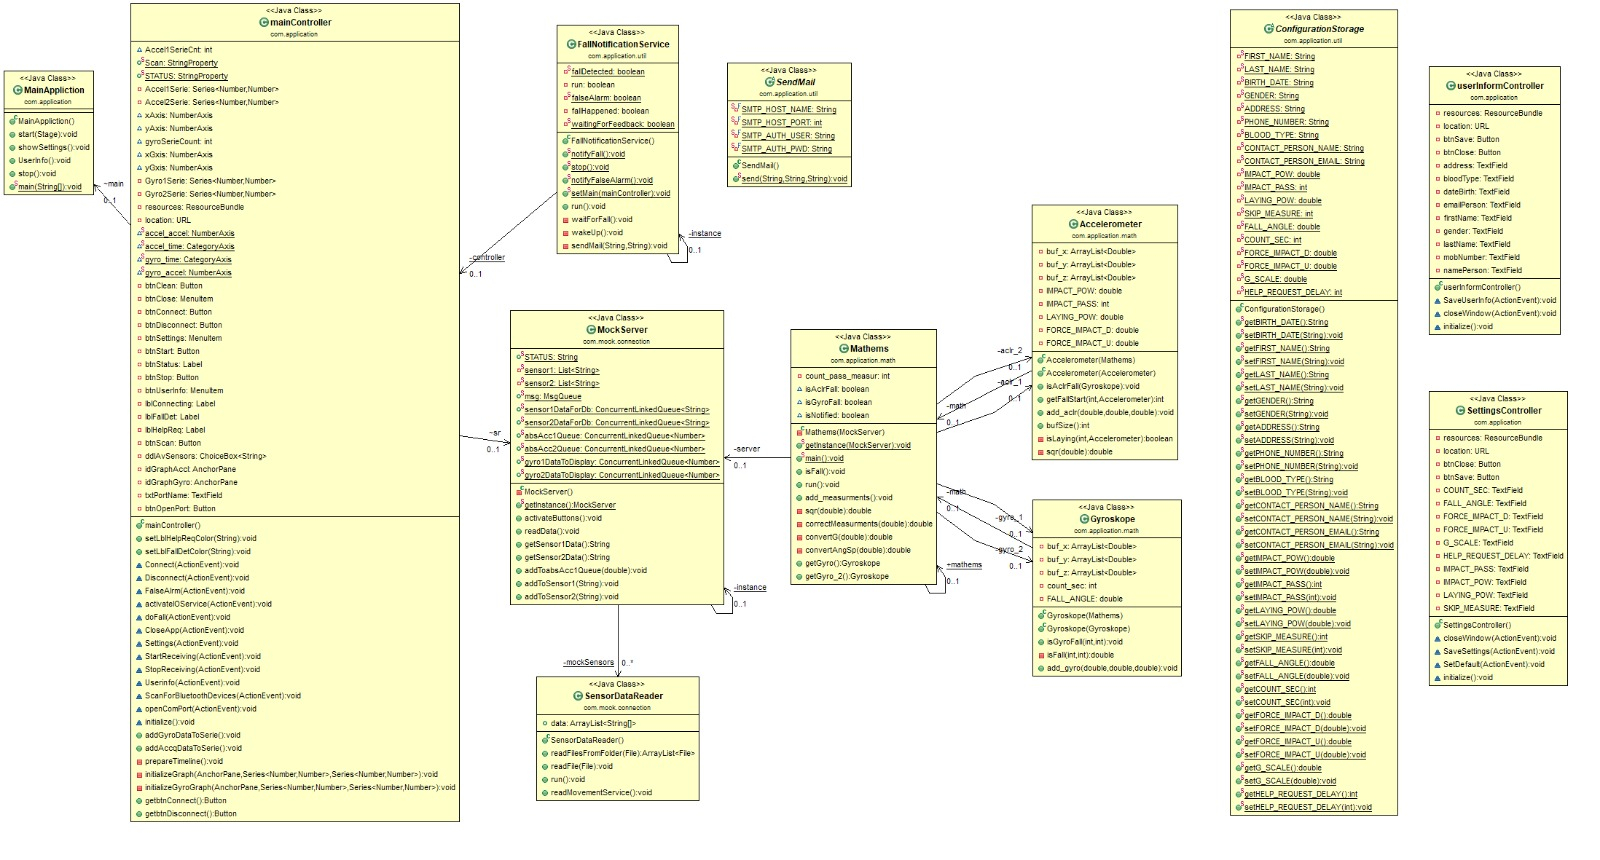
\includegraphics[scale=0.34]{images/UML_Diag.jpeg}
 	\label{img:UML_Diag}
 \end{figure}
 \FloatBarrier
 
 For example, if something in the Mathematical model needs changes, the classes in the other layers require no changes whatsoever to ensure that the application still works. Low complexity and high cohesion is one of the basics of good code, allowing the application to be easily changed and mantained in the future. However, achieving this was no easy feat, as it requires separating the process itself into multiple single-responsibility processes for each task. \\\\\\\\\\\\\\\\\\\\\\\\\\\\\\\\\\\\\\\\\\\\\\\\\\\\\\\\\\\\\\\\\\\\\\\\\\\\\\
 The final version of the application is a Real Time System, with multiple threads that are completely separate from each other. In order for these threads to work as intended, special attention needs to be paid to the order of execution of each class. Without going in depth, first we start the Reader thread, then immediately after without delay the Mathematics thread (part of class Mathems), and lastly the silent Fall Detection thread, which only "wakes up" when a fall event is triggered.
Below is a UML Diagram of all the classes and their interactions.



\clearpage
MockServer will check whether we have new data, SensorDataReader will analyze the file and read the next line if it exists. If yes it will save the data to the MockServer, where it is trimmed and converted into an array of string arrays (two dimensional array). \\\\
\FloatBarrier
\begin{figure}[!h]
	\centering
	\caption{UML Diagram}
	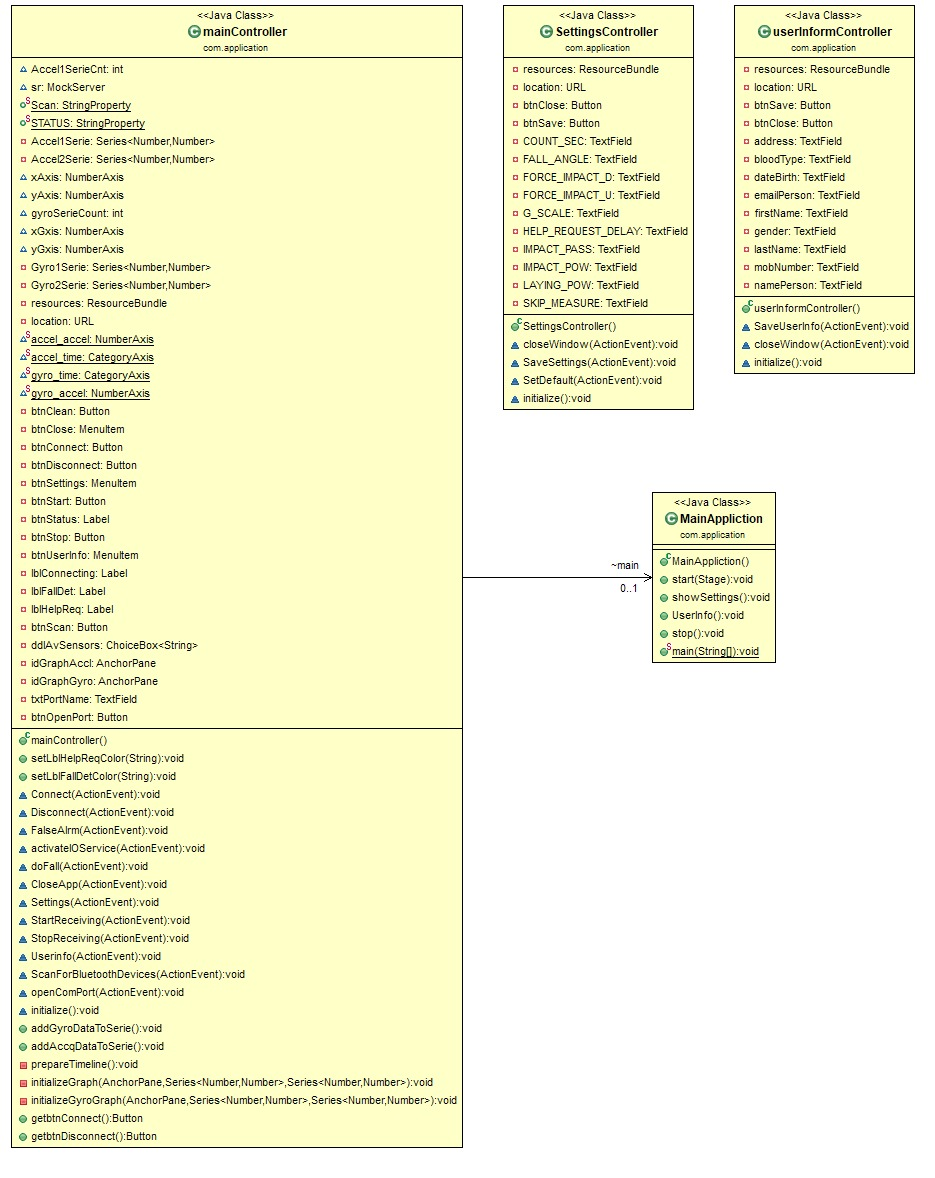
\includegraphics[scale=0.42]{images/UML1.jpeg}
	\label{img:UML1}
\end{figure}
\FloatBarrier

Mathems will analyze the measurements and if it is a Fall will trigger FallNotificationService to send for help.\\ If the False Alarm button is pressed by the User, the process is stopped. If it is pressed after the process is complete, it will send a false alarm notification to the Helper.

\vskip 20cm
\FloatBarrier
\begin{figure}[!h]
	\centering
	\caption{UML Diagram}
	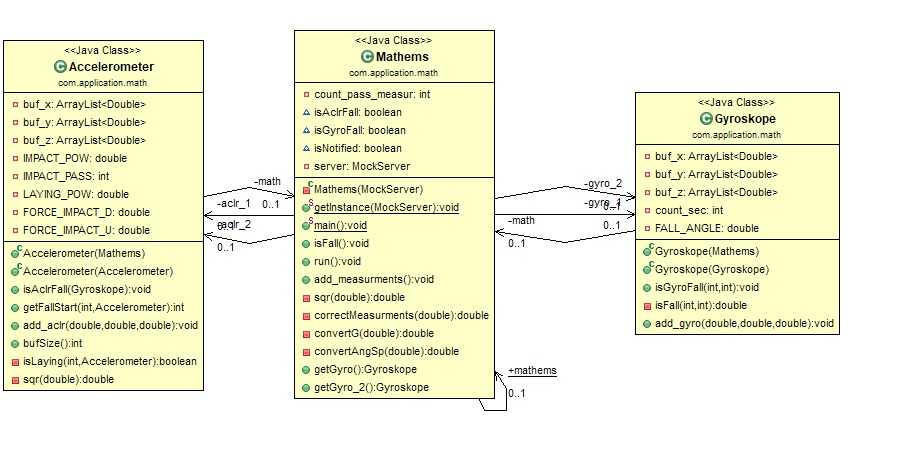
\includegraphics[scale=0.6]{images/UML2.jpeg}
	\label{img:UML2}
\end{figure}
\FloatBarrier
\FloatBarrier
\begin{figure}[!h]
	\centering
	\caption{UML Diagram}
	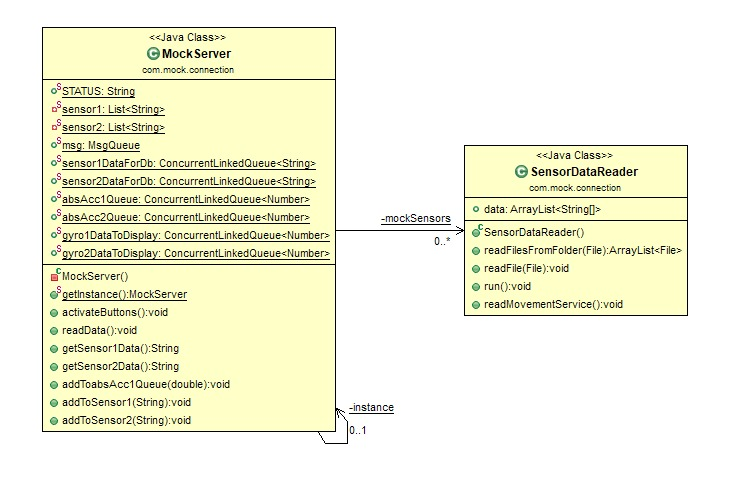
\includegraphics[scale=0.3]{images/UML3.jpeg}
	\label{img:UML3}
\end{figure}
\FloatBarrier

\subsection{Technologies, Libraries, IDEs, Tools}

Below are the different tools used in the making of the application throughout the course of the semester:
\begin{itemize}
	\item Java Programming Language for backend development
	\item JavaFX and SceneBuilder for the User Interface
	\item Gradle to build the project
	\item Eclipse IDE\\\\\\\\\\\\\\\\\\\\\\\\\\\\\\\\\\\\\\\\\\\
	\item ObjectAid UML Explorer for Eclipse to create the UML diagrams from the project structure
	\item \LaTeX \space for reports
\end{itemize}

\section{Measurement Chain}
The application uses pre-recorded sensor data in the form of formatted text files. The data is separated into nine columns for each line. Each three columns represent a single sensor. We have two accelerometers with different resolutions and data ranges and a gyroscope. Each of these sensors has three data points, which correspond to the X,Y,Z axes. The number indicates the force and its direction in the axis. The final force is calculated from these three values separately for each sensor.\\
The measures depend not only on the positioning of the sensors on the individual that recorded the data, but also the person's height, weight, and even factors such as clothing and geographical location. Since there are too many variables to account for and too little time to implement different models for them all, the team opted to allow the configuration of the parameters of a very simple model to better differentiate between different fall-like activities. This can be done easily by the User through the Graphical User Interface\\
We measure indirectly each sensor (the individual sensor information may be found further below)\\
The complete \textit{measurement chain} consists of the sensor data received from the text files and then the conversions applied to it. Since we are not working with actual sensors, no attention needs to be paid to factors such as loss of data (although the model will function reliably regardless) or data corruption due to low connectivity.

\subsection{Accelerometers}
The accelerometers have different respective values for each axis. Their data is vastly different due to the fact that they have different resolutions and data ranges. The first accelerometer (ADXL345) has resolution of 13 bits (8192) and a range of $\pm$16g, while the second one (MMA8451Q) has a resolution of 14 bits (16384) and a range of $\pm$8g. \\
To convert the measurements into G forces we use the formula below:
$$ val = [(2 * Range) / (2^{Resolution})] * AccelerationData \quad g $$
We take that value and apply some variables to make the model more flexible. These variables, which can be changed by the user at runtime, give us the following formula:
$$ a = val \pm e_i \pm e_T \pm e_l \pm e_{cal} \pm e_n \quad g $$
Where \textit{val} is the real value, $e_i$ is the intrinsic error (3\%), $e_T$ is the temperature induced error (0.026\%/$^{\circ}$C), $e_l$ is the non-linearity error (0.5\%), $e_{cal}$ is the initial calibration error (80 mG) and $e_n$ is the noise (8 mG). At room temperature and for the threshold values used by our fall detection algorithm, the above formula can be approximated with:
$$ a = val \pm 6\%  \quad g $$

These are only the default values. Depending on the data set better ranges would apply.

\subsection{Gyroscope}
The gyroscope sensor also has three values total, one for each axis. The way in which this sensor differs from the accelerometers is that the data does not show directional force, but rather angular velocity. Explained blandly, it calculates the rotational force that is applied to the sensor. The data comes from a ITG3200 sensor with a resolution of 16 bits (65536) and a range of $\pm$2000$^{\circ}$/s. \\
The rotational data can be converted to angular velocity using the following formula:
$$ val = [(2*Range)/(2^{Resolution})] * Rotational Data \quad ^{\circ}/s $$
After adding the same variables as we did for the accelerometer, we get the following formula for angular velocity:
$$ v_{ang} = val \pm e_i  \pm e_T \pm e_l \pm e_{cal} \pm e_n \quad ^{\circ}/s $$


\section{Fall Detection Algorithm}
The Fall Detection Algorithm is part of the lowermost layer of the application. After receiving data from the layer directly above, it analyses this data in a FIFO (First In, First Out) manner using ConcurrentQueues. ConcurrentQueues are an implementation of the Queue class that can be used in MultiThreaded applications without causing errors. That is done mostly for safety, as we do not share any of the variables between the threads but rather make extra copies of it. The logic for triggering a fall event is separated in the following classes:
\begin{itemize}
	\item Mathems class - accessor class that communicates with the layer above. It creates instances of the other two classes in the package and uses a thread to convert the data and then store it in separate queues, which are then later used by the classes below.
	\item Accelerometer class - the first class to detect a possible fall. If a fall is suspected, it stores the data that triggered the event and starts the Gyroscope thread to confirm the fall, all while continuing to analyse the G force data passed on from the Mathems class.
	\item Gyroscope class - the main class used to differentiate between falls and normal activities.
\end{itemize}

The Mathems class is the class that takes data from the MockServer class (where the data is stored from the .txt files and converted to an array of strings), parses the data into double values, converts them into Delta G forces and Delta Angular Velocity (for the accelerometer and gyroscope data respectively) and separates them into nine different queues which are used by the Accelerometer and Gyroscope classes. When both classes detect a fall, it calls the Fall Notification service and communicates to the MockServer class that a fall was detected.\\
The Accelerometer class is the first to detect a fall event. If the difference in measurements is above 2g (changeable in the configuration and during runtime in the UI), it switches its own fall detected flag to true and starts the Gyroscope analysis of the data immediately. The accelerometer class implements some aspects of fault control to ensure that outliers in the data do not cause errors in detection.\\
The Gyroscope class has methods that analyse the data and confirm whether the activity detected by the Accelerometer class is a fall or not based on the difference of angular velocity during the moment of impact. If it is above 30 degrees/second we switch the gyroscope fall detected flag to true and send the data that triggered the fall to the Mathems class for display.

\subsection{Configuration Storage}
The different variables that can be changed during runtime (User and Application settings) are stored in the ConfigurationStorage class. This class is fully static and can therefore be called without the need of an instance. All the variables are accessed using get() and set() methods and are connected indirectly to the UI. Most of these values require a knowledgeable user, which is why it is taken for granted that no incorrect values will be passed. However, the type of the passed value could cause the application to crash, therefore we prevent passing incorrect value types (e.g. passing a non-parsable character instead of an integer).

\subsection{Main Thread and Work Logic}
The Mathems class implements the Thread\textsuperscript{\cite{thread}} class from Java. The class first asks the MockServer class for measurements from the SensorDataReader class. If there are no values present, the thread will wait for $10ms$ before requesting again. After waiting, it will make a decision: either add new measurements if they exist and the queue is less then $ConfigurationStorage.getSKIP\_MEASURE()$, or attempt to detect a fall if we have enough values to calculate. \\
To calculate the minimum amount of time for a fall to happen, we can use the kinematic equation:
$$ \vartriangle x = v_0t + \frac{1}{2}at^2 $$
Using the above equation and the assumption that the sensors will be placed on average at around $1m$ from the ground (corresponding to a persons waist), we calculate the minimum time for a fall to be roughly \textit{450ms}.\\ 
The SensorDataReader class passes a new line of values to the MockServer every $5ms$. The function $add\_measurments$ of the Mathems class asks the Server for new measurements with no delay other than the time it takes to receive enough measurements for a fall calculation, then converts them to G and Degree Velocity. Finally, it adds them indirectly through the MockServer into the UI graphs and directly to the corresponding queues for the Gyroscope and the Acclerometer.\\
Furthermore, the class has two flags for the fall: $isAclrFall$ and $isGyroFall$, which are constantly being checked by the Mathems thread. These flags are changed by their respective classes and are initially set to false. If they are both "\textit{true}" when they are checked, the thread calls $FallNotificationService.notifyFall()$. This triggers the fall event which will afterwards send a notification (i.e. email) to the user specified in ConfigurationStorage.

\subsection{Accelerometer}
Every pass of the thread triggers the method $isArclFall$ to start calculations of the Accelerometer. The method makes a copy of objects every time it is triggered and starts in a loop to calculate the absolute value of the impact of all the axes together for every measurement.
\begin{center}
	$impact = \sqrt{Gx^2 + Gy^2 + Gz^2} > 2,$
	$where \quad \textit{Gx, Gy, Gz} \quad are \quad axis $ \\
	$values;$
\end{center}
If the impact is more than $2g$ it is going to check if the patient is lying down to be sure that it was a fall. The Laying function skips several measurements after impact to be sure that the patient is in a static position after the fall. We assume the individual to be lying if the absolute value on the OX and OY axis is between $0.8g$ and $1.3g$.
$$ 0.8 < \sqrt{Gx^2 + Gy^2} < 1.3 $$
If the patient is lying down, the Accelerometer class changes its flag to true. Then the class calls the method of the Gyroscope class to calculate the change in degrees that was registered by patient during the fall. To do this, the Accelerometer class calculates when the fall starts. This is calculated by a function $getFallStart$. The function takes the index of the impact values, subtracts five measurements back and starts one by one to check when the last absolute value on the OZ axis between 0.8 and 1.3 was. This way the application can understand the last index of the measurements when the patient was standing.
$$ 0.8 < \left|Gz\right| < 1.3 $$

\subsection{Gyroscope}
To detect falls correctly and differentiate between fall and nonfall activities, using only the Accelerometers is not enough. It is impossible to tell whether the person actually fell or simply sat down unexpectedly on a sofa. That is why we use the Gyroscope to confirm the fall.\\
The application should store data from the sensors for the Gyroscope the same way as for the Accelerometer class in parallel. Then, the Gyroscope starts to calculate the degrees on OX and OY axes, which were registered by the patient between the beginning of the fall and the impact indexes. \\
To detect whether after a strong enough impact the individual is laying down immobile or not, we need the deegrees on the X and Y axis. Since the sensor instead gives us rotational velocity, we need to convert it using the following formula:\\
\begin{center}
	$angle_i = \left| \frac{Gx_i}{CS} \right| + \left| \frac{Gy_i}{CS} \right|,$\\
\end{center}
where \ Gx,\ Gy\ is\ the\ velocity\ on\ OX\ and\ OY\ axis and CS\ is\ the\ amount\ of\ measurements\ per\ second.\\

Then this value should be divided by 180 and the application should take the remainder of the division and subtract from it 90 degrees. If this value is less than 30 degrees the application changes another flag for "true".
\begin{center}
	${\sum}_i angle_i - 90 \pm 180 * n < 30,$ \\
	$where \quad n \in Z; $
\end{center}

\subsection{Mathematic Fault Control}
To minimize faulty decision making, i.e. detecting falls when there are none and vice versa, we have implemented several ways to ensure that the thread runs correctly and makes the correct decisions. Firstly, we ensure that we only have one instance of the Mathems class by making it a Singleton. That way we do not have multiple threads interfeering with each other. Secondly, we ensure that the Mathems class is initialized second to last, right before FallNotification. This is due to the fact that it requires an instance of MockServer to work, otherwise the application will not start at all (this issue actually prevented progress on the project for a whole week, as the resulting exception does not return a stack trace since the application fails on the first call).\\
Also, we implemented methods to skip certain measurements, such as ones right after a fall is detected. Due to the way forces work, an individual can "bounce" for a few milliseconds right after a fall, meaning the sensors would still register movement and incorrectly classify the person as still being active. Since multiple measurements are used in detecting a fall, singular outliers caused by erroneous data will not cause an issue in fall detection. For a fall to be detected, 30 measurements need to follow a pattern that can only be caused by a real fall. 

\section{Development and Application Fault Control}
\subsection{Fall Notification Service (FNS)}
This is the service that handles the notifications triggered by the detection of a fall. Its code interacts with each and every other part of the desktop application and offers a good overview of its main features.\\
On start the FNS idles while waiting for a trigger. When the fall detection algorithm thinks the user has fallen, it alerts the FNS which raises the "Fall Detected" flag in the GUI and then waits for a preset amount of time (default 10 seconds) for feedback from the user in the form of a button press on the UI. If no such feedback comes, help is requested (an email is sent to the helper’s address) and the "Help Requested" flag is raised in the GUI. Instead, in case a button is pressed before the preset time has elapsed, the "Fall Detected" flag lowered, after which the cycle repeats itself. The user can also signal a false alarm after help has been already request (that is, when in the "Wait" state): in this case all flags are lowered and a new message is sent to the helpers explaining that it was indeed a false alarm.\\
Below you see a state machine diagram illustrating the service operation:
\FloatBarrier
\begin{figure}[!h]
	\centering
	\caption{Fall Notification Service}
	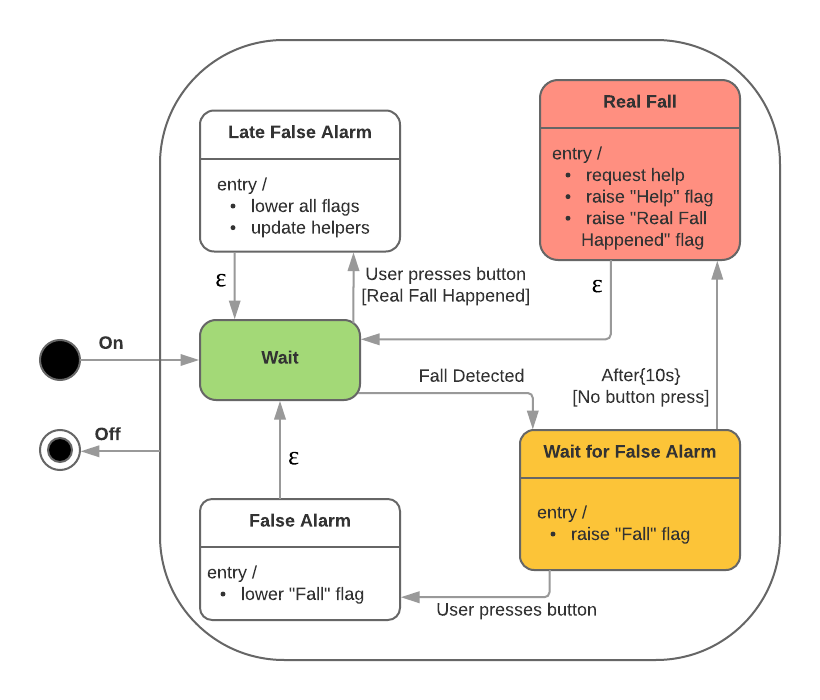
\includegraphics[scale=0.3]{images/FNS.png}
	\label{img:FNS}
\end{figure}
\FloatBarrier
The content of the messages sent to the helpers, as well as the addresses of the helpers themselves, can be changed through the GUI. The waiting time after a fall is detected and before help is requested, can also be modified in the same way.


\subsection{Graphical User Interface} 
To implement GUI based on the mock up made earlier, JavaFX Scene Builder\textsuperscript{\cite{JavaFX}} was used. JavaFX Scene Builder is a tool that lets users design a JavaFX application’s UI. UI components can be
draged and dropped to a work area, modify their properties and at the end we will have FXML code
for the created layout generated automatically. The result is a FXML file that can be combined with a Java project by binding the UI to the applications logic.\\
In the first version of GUI we have main window with area for Accelerometer and Gyroscope graphs
and buttons to establish and control the connections to the SensorTags.\\
Through the File menu the user can access the User General Information and Settings windows.
In User General Information the user should fill in the form with his data and the contact person‘s data.\\
In Settings menu the calibration values for the fall detection algorithm can be inserted.

\subsection{Fault Control}
We implement a mix of different fault control techniques for the application depending on several factors. For issues that would crash the application we use a mix of good coding practices and error handling. The most important practice is disallowing the passing of null variables. We do this by copying values instead of sharing them between multiple threads (although this is unnecessary, in our application it is acceptable as we are not concerned about memory usage), forcing the order of execution to go a certain way (instantiate Mathems and SensorDataReader after the MockServer and Main class) and also preventing the User from actions that would result in such values being passed. \\
Preventing application crashing actions from the User is the main way we ensure that the application will not fail. While we do expect the User to be knowledgeable in the area and the use of this application, we do not expect them to be a programmer. Therefore, actions that would cause exceptions are either disregarded if they are not critical (non properly formatted text file is selected, resulting in nothing happening when the Start button is pressed), handled when they cause exceptions but are not critical (a non properly formatted text would cause incorrect data to be passed to the queues), or outright prevented if they are absolutely critical to the runtime of the application (e.g. User can only select .txt files).\\
An interesting problem is that whenever we press Start we start the SensorDataReader thread, and when we press Stop we close it and delete it. Pressing Start twice would create multiple threads based on the same file, therefore after the User presses Start the button is disabled. It is re-enabled once the User presses the Stop button.\\
For debugging purposes we added two extra buttons, one to trigger a Fall event and one to call a FalseAlarm. As they simply call static methods indirectly, they do not interfeere during runtime at all.

\nocite{*}
%----------------------------------------------------------------------------
% Bibliography
%----------------------------------------------------------------------------	
\printbibliography
\end{document}
%----------------------------------------------------------------------------
